  \documentclass[11pt]{article}

\usepackage[utf8]{inputenc}

\usepackage{graphicx}
\graphicspath{{assets/}}
\usepackage[francais]{babel}
\usepackage{listings}
\usepackage{float}
\usepackage[toc,page]{appendix}

%https://mysnippets443.wordpress.com/2015/11/28/latex-insert-javascript-code-with-lstlisting-package/


%Define the listing package
\usepackage{listings} %code highlighter
\usepackage{color} %use color
\definecolor{mygreen}{rgb}{0,0.6,0}
\definecolor{mygray}{rgb}{0.5,0.5,0.5}
\definecolor{mymauve}{rgb}{0.58,0,0.82}
 
%Customize a bit the look
\lstset{ %
backgroundcolor=\color{white}, % choose the background color; you must add \usepackage{color} or \usepackage{xcolor}
basicstyle=\footnotesize, % the size of the fonts that are used for the code
breakatwhitespace=false, % sets if automatic breaks should only happen at whitespace
breaklines=true, % sets automatic line breaking
captionpos=b, % sets the caption-position to bottom
commentstyle=\color{mygreen}, % comment style
deletekeywords={...}, % if you want to delete keywords from the given language
escapeinside={\%*}{*)}, % if you want to add LaTeX within your code
extendedchars=true, % lets you use non-ASCII characters; for 8-bits encodings only, does not work with UTF-8
frame=single, % adds a frame around the code
keepspaces=true, % keeps spaces in text, useful for keeping indentation of code (possibly needs columns=flexible)
keywordstyle=\color{blue}, % keyword style
% language=Octave, % the language of the code
morekeywords={*,...}, % if you want to add more keywords to the set
numbers=left, % where to put the line-numbers; possible values are (none, left, right)
numbersep=5pt, % how far the line-numbers are from the code
numberstyle=\tiny\color{mygray}, % the style that is used for the line-numbers
rulecolor=\color{black}, % if not set, the frame-color may be changed on line-breaks within not-black text (e.g. comments (green here))
showspaces=false, % show spaces everywhere adding particular underscores; it overrides 'showstringspaces'
showstringspaces=false, % underline spaces within strings only
showtabs=false, % show tabs within strings adding particular underscores
stepnumber=1, % the step between two line-numbers. If it's 1, each line will be numbered
stringstyle=\color{mymauve}, % string literal style
tabsize=2, % sets default tabsize to 2 spaces
title=\lstname % show the filename of files included with \lstinputlisting; also try caption instead of title
}
%END of listing package%
 
\definecolor{darkgray}{rgb}{.4,.4,.4}
\definecolor{purple}{rgb}{0.65, 0.12, 0.82}
 
%define Javascript language
\lstdefinelanguage{JavaScript}{
keywords={typeof, new, true, false, catch, function, return, null, catch, switch, var, if, in, while, do, else, case, break},
keywordstyle=\color{blue}\bfseries,
ndkeywords={class, export, boolean, throw, implements, import, this},
ndkeywordstyle=\color{darkgray}\bfseries,
identifierstyle=\color{black},
sensitive=false,
comment=[l]{//},
morecomment=[s]{/*}{*/},
commentstyle=\color{purple}\ttfamily,
stringstyle=\color{red}\ttfamily,
morestring=[b]',
morestring=[b]"
}
 
\lstset{
language=JavaScript,
extendedchars=true,
basicstyle=\footnotesize\ttfamily,
showstringspaces=false,
showspaces=false,
numbers=left,
numberstyle=\footnotesize,
numbersep=9pt,
tabsize=2,
breaklines=true,
showtabs=false,
captionpos=b
}



\begin{document}
\renewcommand{\appendixtocname}{Annexes}
\renewcommand{\appendixpagename}{Annexes}
\renewcommand{\refname}{Sources}



\title{Candide 2.0 ou l'optimisme en jeu vidéo }
\author{Nina Ionescu 3mg01 \\ Mentor : Jean-Marc Ledermann \\ Lycée Denis de Rougemont}
\date{}
\pagenumbering{gobble}
\maketitle

\includegraphics{title}
\newpage
\tableofcontents
\newpage
\pagenumbering{arabic}
\section{Introduction}\
\textit {Il y avait en Westphalie...} Et si cet incipit mythique se retrouvait un jour pixelisé, cela donnerait quoi ? C'est ce à quoi j'ai essayé de répondre lors de ce travail de maturité, qui consistait à adapter le premier chapitre dans \textit{Candide} de Voltaire en un jeu vidéo de type RPG (jeu de rôle).
% mettre des screenshots et ue brève explication du jeu plus références à Candide
\begin{figure}[h]

\includegraphics[scale=0.33]{ecranTitre}
\centering
\end{figure}
\subsection{Lexique}
Afin d'avoir une meilleure compréhension de ce document, voici un lexique. \\
\begin{itemize}{}{}
\item \textbf{assets} : Désigne l'ensemble des fichiers visuels et auditifs du jeu.
\item \textbf{frame}: Image constituant une partie de l'animation d'un sprite.
\item \textbf{hp}: Abréviation de health points, points de vie.
\item \textbf{map}: Carte.
\item \textbf{overworld}: Monde extérieur en français. Désigne l'ensemble de maps constituant le jeu.
\item \textbf{pixel art} : Style graphique inspiré des jeux rétros où les assets sont dessinés à la main en respectant certains formats.
\item \textbf{pnj}: Abréviation de personnage non-jouable.
\item \textbf{Phaser} : Nom de la librairie utilisée pour ce projet. Un objet Phaser est un objet créé à partir des classes de la librairie.
\item \textbf{signal} : Objet Phaser qui gère les événements et leur enclenchement.
\item \textbf{sprite}: Image du jeu en partie transparente capable de déplacement.
\item \textbf{spritesheet}: Image regroupant les frames d'animation d'un sprite.
\item \textbf{state} : Section du jeu. Objet issu de la classe \textit{State} de Phaser.
\item \textbf{tile} : Carreau en français; petite image carrée à texture répétée.
\item \textbf{tilemap}: Carte à carreaux en français. Carte du jeu formée par des tiles.
\item \textbf{tileset}: Ensemble de tiles sous forme de spritesheet.
\item \textbf{warp}: Zone qui une fois pénétrée déclenche un changement de map.
\end{itemize}

\subsection{Travail réalisé}
Lors de ce projet, une relecture attentive de Candide a été réalisée pour récolter tout ce qui peut servir à une adaptation. J'ai programmé de nombreuses classes et méthodes qui servent d'outils pour la construction du jeu ainsi que quelques fonctions uniques pour que l'histoire prenne place. En parallèle à cela, j'ai dessiné les spritesheets pour les personnages et les décors, tout ce qui sert d'élément de jeu (bulles, conteneurs de texte, ...), une police de caractères et réalisé les maps. Un travail sur de la musique a aussi été envisagé et quelques ébauches musicales pour le jeu ont vu le jour, bien qu'inexploitées dans le rendu final.

\section{Conception du jeu}

\subsection{Projet original}
Le but du projet original était d'adapter l'entièreté de Candide sous forme de jeu vidéo avec un scénario alternatif et créer tous les assets visuels et auditifs. Le tout en 6 mois, un projet qui aurait été qualifié de totalement réaliste par la pointe d'ironie de Voltaire et celle de mon mentor avisé...\\

Dans ce projet, le joueur pourrait incarner Candide et vivre une aventure propre aux choix qu'il serait amené à faire durant le jeu. Il dialoguerait avec les personnages qui proposeraient des quêtes à remplir et influenceraient le jeu, il collecterait des objets trouvés le long de son voyage pour les revendre ou les utiliser lors de combats à l'épée ou philosophiques. Il récolterait une collection de graines pour les planter au final dans son jardin... Le tout agrémenté de belles cinématiques.\\ Le jeu n'aurait pas forcément été agréable avec le joueur, le but étant que ce dernier ressente ce qu'a ressenti Candide lors de son périple. Un exemple de choix qui avait été imaginé était  que le joueur ait le choix très tôt dans le jeu de choisir combien de sucre il souhaite dans son thé. Un choix apparemment innocent qui aurait révélé ses conséquences beaucoup plus tard dans le jeu, lorsque Candide rencontre l'esclave qui travaille pour la production de sucre. En fonction de la réponse du début, l'esclave sera plus ou moins maltraité. 


\subsection{Résultat final}
Après avoir réalisé que créer un jeu vidéo n'était pas simple, le projet a été réduit pour adapter uniquement le premier chapitre du livre. 
% personnages , dessiner
%organisation du code
%explique que les extraits sont des extraits
Le joueur incarne donc Candide et peut se promener des décors inspirés de l'incipit. Il peut dialoguer avec les pnjs présents dans les décors et faire des combats avec certains d'entre eux.
\begin{figure}[H]
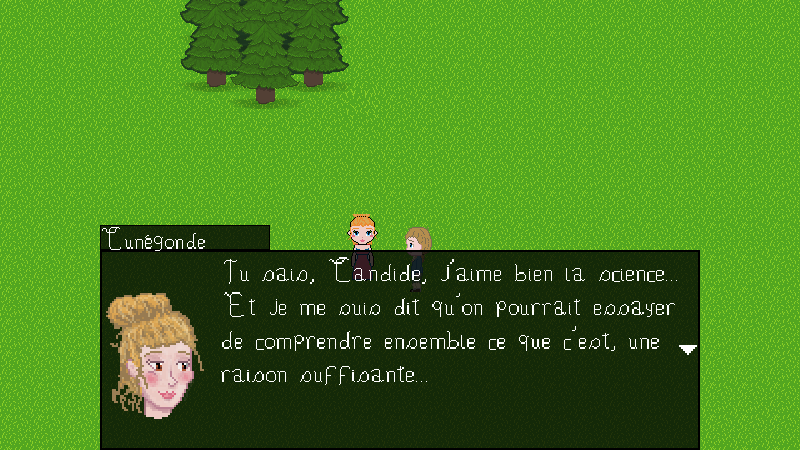
\includegraphics[scale=0.33]{cunegondeScn}
\centering
\end{figure}
\subsection{Adaptation}
L'adaptation est quelque chose de primordial. Comment donner une apparence physique à un personnage ? Le faire parler ? Créer un environnement pour le joueur ? Le meubler ?\\ 
Tous les assets sont une interprétation de l'œuvre originale. Par exemple, le design de Pangloss doit faire comprendre immédiatement au joueur que c'est un intellectuel trop sûr de lui. Il porte des lunettes pour accentuer le stéréotype du savant et pour illustrer son discours. Le sprite est déjà marqué de quelques traits de vieillesse, ce qui accentue la "sagesse" de Pangloss. Il plisse des paupières en souriant de coin, ce qui révèle sa confiance. Tout ceci doit transparaître en seulement quelques pixels.
\begin{figure}[H]

\includegraphics[scale=0.8]{panglossHead}
\centering
\end{figure}
Le personnage de Candide doit faire transparaître de la naïveté, de l'innocence et un peu de maladresse. Ces éléments sont représentés avec ses mèches en bataille et sa chemise à moitié rentrée dans ses chausses, ainsi qu'avec son sourire gentil.\\
\begin{figure}[H]

\includegraphics[scale=1.3]{candide}
\centering
\end{figure}
De même que le décor : Il y a la cour et le château. Le château \textit{avait une porte et des fenêtres} et il est fait de pierres taillées. Pour illustrer une part d'ironie de Voltaire, quelques pierres sont irrégulières, voire manquantes.
\begin{figure}[H]
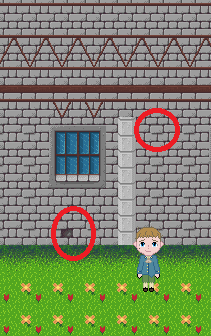
\includegraphics{chateau}
\centering
\end{figure}

Malheureusement, le décor n'est pas complet à cause du temps que la création prend. Il est également difficile de créer un jeu sans décor dessiné au préalable.\\



%plus d'exemple si temps

\section{Déroulement du jeu}
%expliquer les dialogues, conserver le contenu tout en l'adaptant etc...donner des exemples de situations alternatives . et le résultat actuel
%expliquer la complication lié au temps, le rabotage etc..
Tout commence dans la cour du château de monsieur le Baron de Thunde-ten-tronckh où les fleurs de son jardin se balancent au vent. Le joueur peut se diriger pour parler à Pangloss.
\begin{figure}[H]
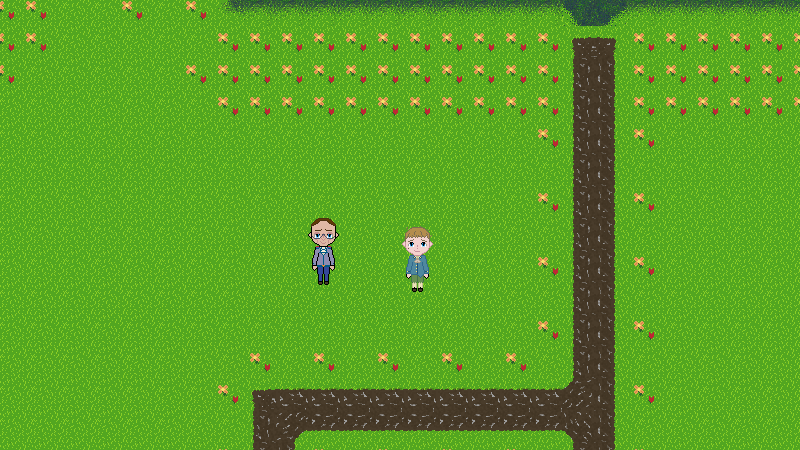
\includegraphics[scale=0.35]{gameplay1}
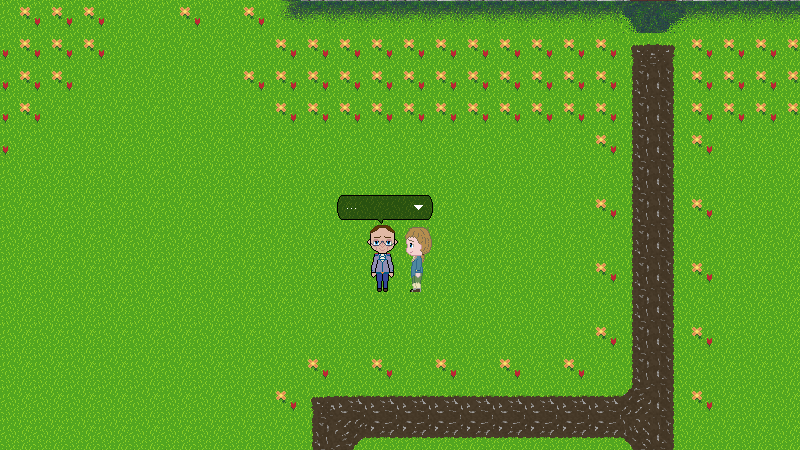
\includegraphics[scale=0.35]{gameplay2}
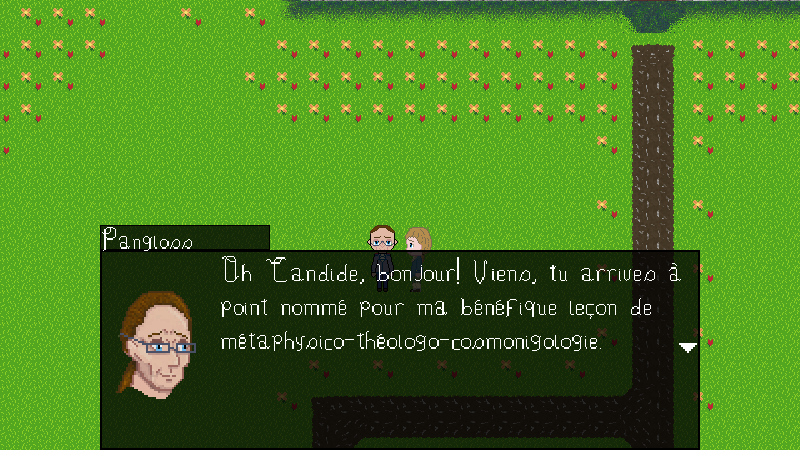
\includegraphics[scale=0.35]{gameplay3}
\centering
\caption{première rencontre avec Pangloss}
\end{figure}
Pangloss illustre son célèbre discours qui fait de lui un grand philosophe puis demande au joueur de faire son premier choix : agréer de répondre toujours positivement ou non. \\

\begin{figure}[H]
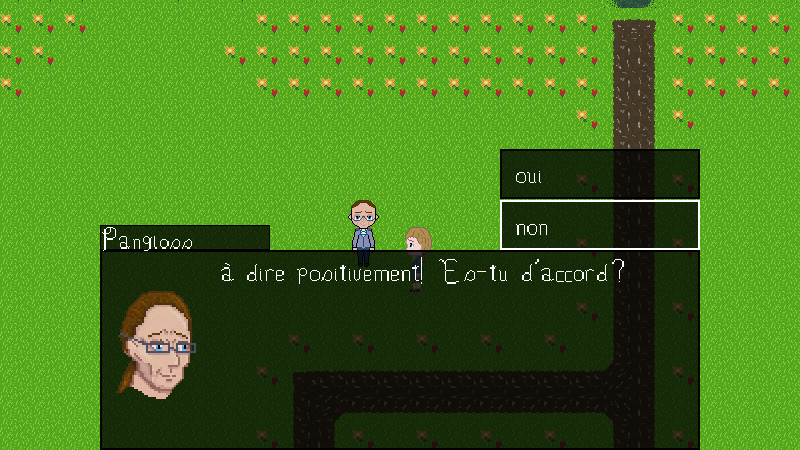
\includegraphics[scale=0.35]{choix}
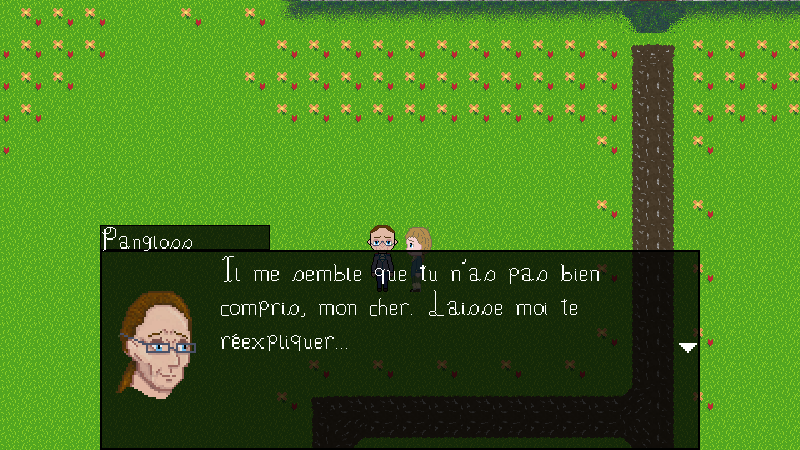
\includegraphics[scale=0.35]{gameplay4}
\centering
\caption{les conséquences de la réponse négative}
\end{figure}

Le long discours rébarbatif de Pangloss sert à accentuer le côté désagréable du personnage, surtout si le joueur refuse de toujours répondre positivement. \\

Le joueur est libre de se promener dans l'environnement pour y rencontrer quelques personnages.

\begin{figure}[H]
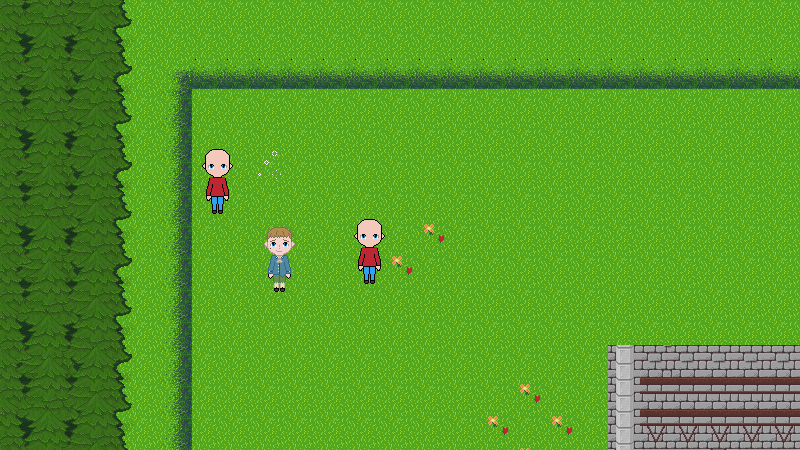
\includegraphics[scale=0.35]{gameplay5}
\caption{2 pnjs}
\end{figure} 

Celui du haut propose un combat à l'épée. Le joueur peut l'accepter quand il en a envie. 

\begin{figure}[H]
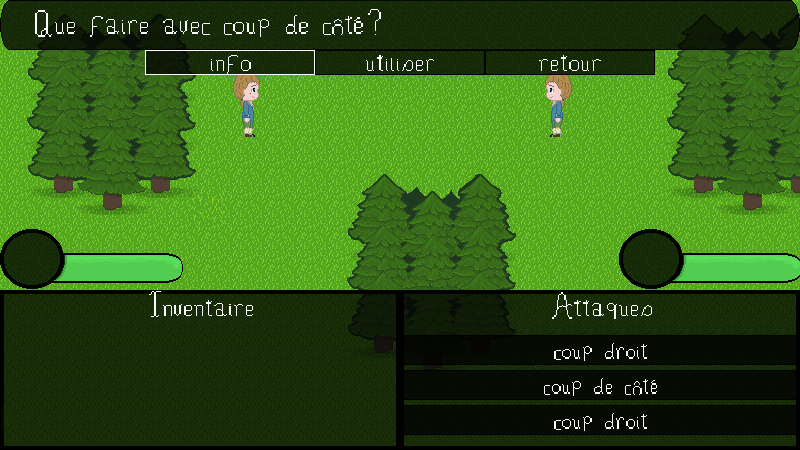
\includegraphics[scale=0.35]{gameplay6}
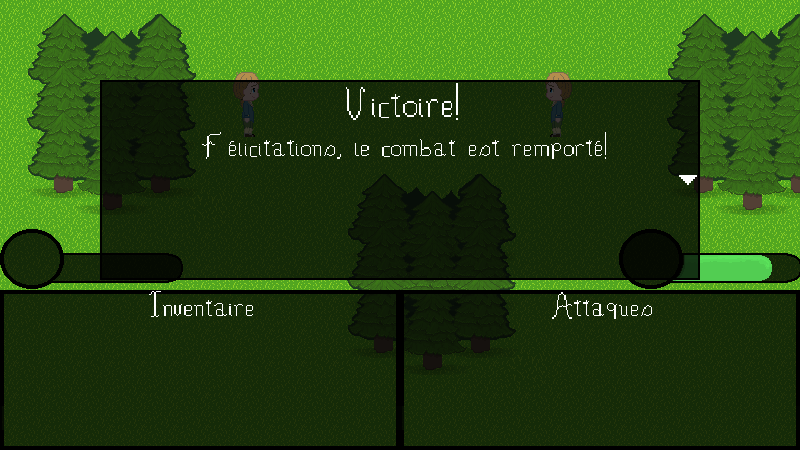
\includegraphics[scale=0.35]{gameplay7}
\centering
\caption{déroulement du combat}
\end{figure}

Le joueur peut également aller voir Cunégonde dans le petit bois, appelé parc, à gauche du château.

\begin{figure}[H]
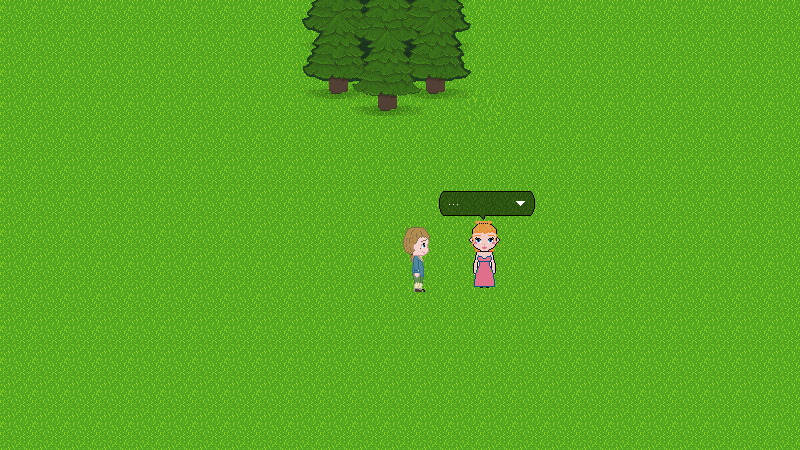
\includegraphics[scale=0.35]{gameplay8}
\centering
\caption{rencontre avec Cunégonde}
\end{figure}

Enfin, il peut retourner au château, où il rencontrera Paquette.

\begin{figure}[H]
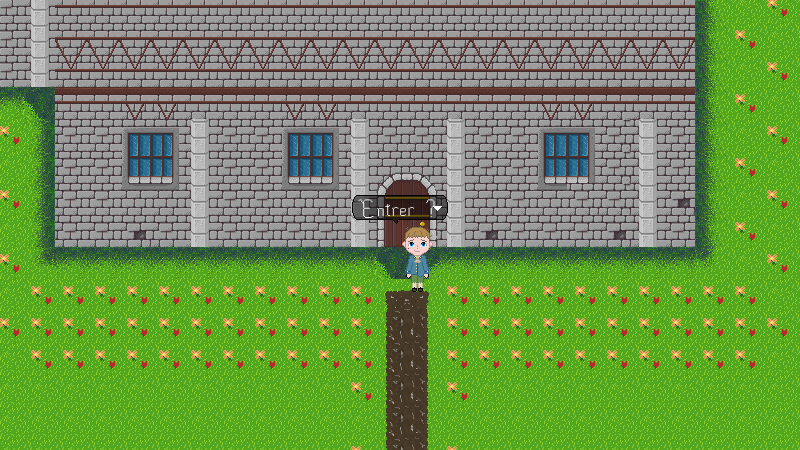
\includegraphics[scale=0.35]{gameplay9}
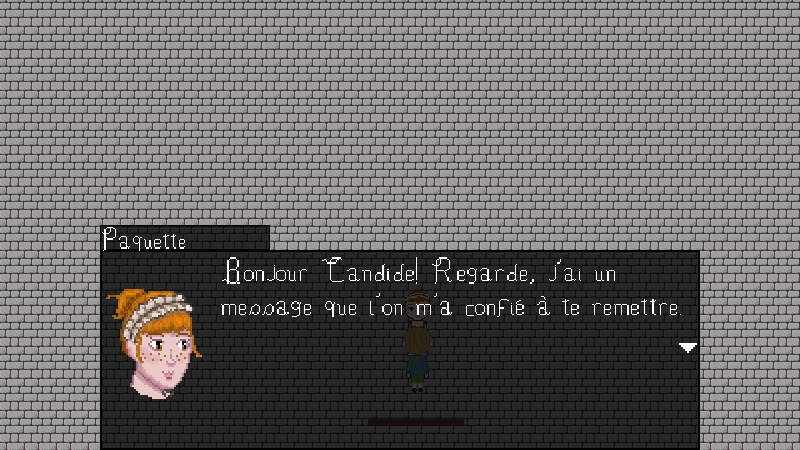
\includegraphics[scale=0.35]{gameplay11}
\centering
\caption{Au château}
\end{figure}

C'est déjà la fin de cette petite démonstration. 
\begin{figure}[H]
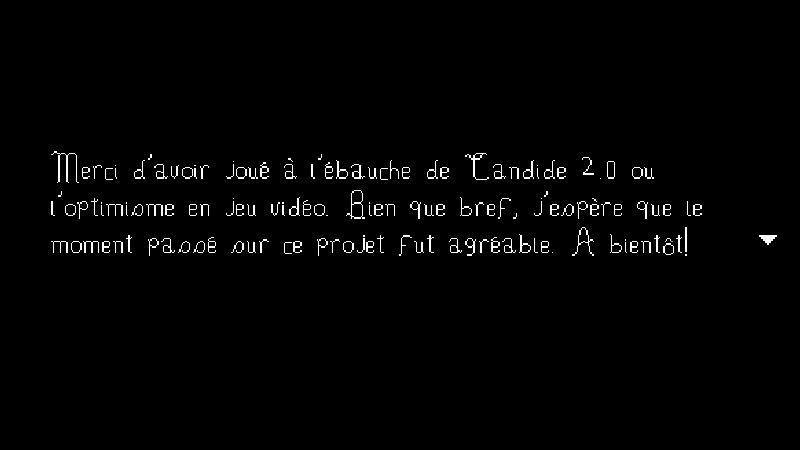
\includegraphics[scale=0.35]{gameplay12}
\centering
\caption{message de fin}
\end{figure}

Pour recommencer à jouer, il faut rafraîchir la page.



\section{Fonctionement du code}
Ce projet a été réalisé en JavaScript, avec les additions de ECMAScript6 et de deux librairies conçues pour la réalisation de jeu-vidéo : Phaser.js ainsi que Phaser-tilemap-plus.js . La majorité du code comprend des objets et des classes créés afin de pouvoir les utiliser comme outils de création.\\

\subsection{Balayage du code}


\subsection{En résumé}
Beaucoup de code pour au final, un petit rendu. En effet, programmer un jeu de type RPG est beaucoup plus compliqué que prévu. Chaque fonction pour la progression du jeu est unique et il est très difficile d'avoir ne serait-ce qu'un minimum de scénario. Le niveau de complexité est déjà assez élevé rien qu'en programmant un long dialogue qui ne sera affiché qu'une fois au cours du jeu, comme par exemple les quelques lignes de Pangloss. Ce à quoi mon projet s'approche le plus est peut-être une situation de base inspirée du premier chapitre de Candide, mais il est loin d'être proche d'un jeu. Pourtant tout ce qui a été programmé est indispensable pour chaque jeu vidéo de type RPG car ce sont les éléments de base pour le construire. Le code est quelque chose d'invisible pour le joueur et il peut être très frustrant de constater qu'après tant de code écrit, seul un petit résultat est affiché à l'écran. \\

Certains éléments qui ont été programmés mériteraient d'être réécrits avec les connaissances acquises lors de ce projet. En effet, les premiers programmes ont été créés en découvrant encore Phaser, ils n'exploitent donc pas forcément toutes les fonctionnalités Phaser qui permettent parfois d'avoir un code plus simple, propre et efficace.\\
\section{Scénario alternatif}
Cette section va brièvement présenter les idées de bases pour le jeu ainsi que le travail effectué sur le scénario. Ce travail a été réalisé tôt dans la durée du projet, lorsque l'espoir de réaliser un jeu complet était encore à l'horizon. Malheureusement, il ne fait pas encore l'objet de la réalisation en ce moment, mais il servira de canevas pour le futur.\\

%expliquer les dialogues, conserver le contenu tout en l'adaptant etc...donner des exemples de situations alternatives . et le résultat actuel, expliquer la complication lié au temps, le rabotage etc.. relevé dans le livre
\section{Conception des assets}
\subsection{Visuel}
%logiciels utilisé , techniques(travailler avec des tiles, couches de transparence...)inspiration pour les personnages, dessins originaux etc.. restrictions au niveau du pixel art, base pour cohérence etc...
Tous les dessins ont été réalisés avec le logiciel Pyxel Edit et les maps avec le logiciel Tiled.
\subsubsection{Police personnalisée}
%comment on a fait
La police du jeu est une police conçue pour le projet. En effet, Phaser permet d'afficher du texte de manière assez simple avec des polices standards, le problème est que les polices décadrent avec l'ambiance du jeu. Phaser permet aussi d'afficher du texte avec des polices bitmap. Il était également possible d'en choisir une déjà existante et de créditer son auteur mais aucune police ne correspondait aux attentes. La meilleure solution était donc de créer une police personnalisée, qui intègrerait sans problème le style graphique du jeu. \\

Pour créer la police, deux sites ont étés utilisés, calligraphr.com ainsi que kvazars.com/littera.\\ Calligraphr permet de télécharger un modèle à remplir avec les lettres souhaitées puis de convertir ensuite ces images en police de format trueTypeFont. Grâce à Littera, il est ensuite possible de convertir cette police en police bitmap pour être utilisée dans le jeu. \\

Un des problèmes rencontrés en cours de réalisation était la précision du rendu. Il fallait utiliser des équivalent de pixels, des carrés de 11X11px pour avoir un rendu pixelisé car les modèles de Calligraph font la grandeur d'une feuille A4. \\
Un autre problème était le rendu avec Littéra. En effet, le site a appliqué un filtre d'anti-alias automatiquement sur les lettres, ce qui gâchait l'effet du pixel art. Il a donc fallu retoucher toute les lettres à la main sur l'image finale. En cours de la réalisation, plusieurs lettres ont du être ajoutées, ce qui a eut comme effet de modifier la disposition des lettres sur la feuille finale et donc de devoir recommencer le travail fastidieux de les redessiner. 
\subsubsection{Sprites de dialogues}
%techniques(couches, dessins - restrictions), exemple , projet noir blanc

Pour garder une cohérence stylistique ainsi que pour simplifier le travail, tous les sprites de dialogues ont une base commune de 35X67 pixels: 
\begin{figure}[H]
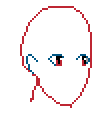
\includegraphics{base}
\centering
\end{figure}
Ensuite, les traits caractéristiques de chaque personnage sont dessinés par dessus cette base. Seuls quelques pixels servent à changer totalement l'expression d'un personnage. Ces traits sont donc primordiaux pour donner une individualité aux personnages. Il faut que le joueur ressente leur caractère au premier regard. Voici un recueil des traits principaux des personnages dont quelques visages sont déjà familiers.\\
\begin{figure}[H]
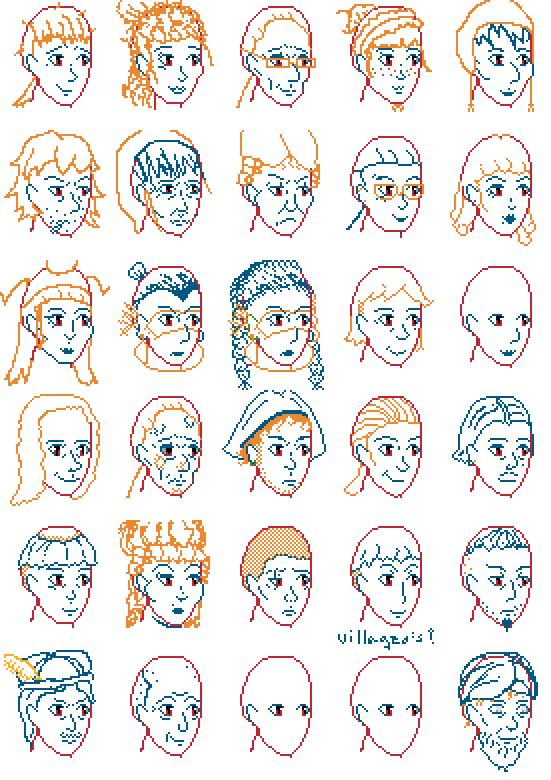
\includegraphics[scale=0.7]{faces_Candide}
\centering
\caption{Ebauche des personnages.}
\end{figure}
De gauche à droite :\\\textit{première colonne} : Candide , Cunégonde, Pangloss, Paquette, Cacambo\\
\textit{deuxième colonne}: Martin, la vieille, le baron de Thunder-ten-Tronckh, moi-même, la marquise de Parolignac\\
\textit{troisième colonne} :  Une fille de l'Eldorado, un Oreillon, une Oreillonne, Jacques le bienfaiteur\\
\textit{quatrième colonne} : Voltaire, Pangloss atteint de la syphilis, meneer Vonderdendur, le frère de Cunégonde,signore Poccocurante\\
\textit{cinquième colonne} : frère Giroflée, la baronne de Thunder-ten-Tronckh, l'esclave de Vonderdendur, un potentiel villageois , l'inquisiteur de Lisbonne \\
\textit{sixième colonne} : le roi des Bulgares, l'abbé périgourdin, le vieux Turc\\

Cette illustration montre la richesse du pixel art, les personnages sont cohérents entre eux pourtant ils ont chacun leur propre design.\\

Une fois la base créée, l'animation est dessinée en modifiant la frame pour créer le mouvement des paupières et des lèvres du personnage. Les couleurs de bases sont ensuite définies sur une couche en dessous des contours puis les détails sont rajoutés en transparence sur une couche supérieure. 
\begin{figure}[H]
\includegraphics[scale=1.5]{exempleTM}
\centering
\caption{La marquise de Parolignac en cours de réalisation}
\end{figure}

Chaque sprite demande un travail considérable , il faut donc énormément de temps pour illustrer chaque personnage unique de Candide. Pour les personnages qui servent uniquement à habiter le décor, une solution a été pensée : dessiner quelques alternatives physiques ( diverses coupes de cheveux, nez, bouches,...) en niveaux de gris puis les associer à une couleur. Il sera alors beaucoup plus simple de recolorer et d'associer différentes parties pour recycler une partie du travail effectué.\\
La technique des niveaux de gris a été appliquée pour les barres de vies lors des combats, car il aurait été trop compliqué de coder en prenant compte 3 images distinctes. Malheureusement, cette technique n'a pas encore été testée pour la réalisation de personnage.
\subsubsection{Sprites d'overworld}
%techniques, exemples
Tous les sprites de ce type ont également une base commune.
\begin{figure}[H]
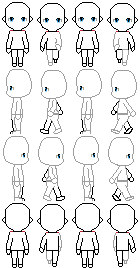
\includegraphics[scale=1]{animationBase}
\centering
\end{figure}
L'animation de marche a été assez difficile à dessiner car il fallait que le résultat semble fluide et naturel.\\

Ces sprites reprennent les plus gros détails des personnages et ont un coloriage plus minimaliste. Plus de détails pourraient être cependant ajoutés.
\begin{figure}[H]

\includegraphics[scale=1.5]{panglossSprite}
\centering
\end{figure}
\subsubsection{Tilesets}
%techniques, exemples
\subsubsection{Tilemap}
\subsection{Musical}
%logiciel utilisé , techniques (trouver une suite d'accord, les instruments etc..) , éventuellement les bruitages , la campanella midi file
Le logiciel Bosca Ceoil a été utilisé pour créer des ébauches musicales qui ne figurent pas dans le projet final. Il n'est pas facile de composer une musique qui sied bien à l'atmosphère d'un jeu vidéo. Les musiques de l'opéra Candide de Bernstein auraient pu être utilisées mais transcrire une musique est très compliqué et les fichiers midis trouvés n'avaient pas un joli rendu.\\

Étant cependant une grande admiratrice de Paganini, la Campanella a été choisie comme musique accompagnatrice du jeu. Un fichier midi a été utilisé avec Bosca Ceoil et le tout avait un rendu agréable.  
\subsection{En résumé}
Encore une fois, beaucoup de travail pour un petit résultat. Le pixel art demande beaucoup de patience et créer un univers cohérent et agréable visuellement est difficile sans assets complets. Malheureusement, une partie des assets n'est pas encore utilisée dans le projet rendu. En effet, ayant pensé avoir le temps de développer plus d'histoire, d'autres personnages ont été dessinés au début du projet. Ils figureront tout de même en annexe.
\section{Conclusion}
\subsection{Nina Ionescu ou l'optimisme} 
Ah, que dire de la naïve candeur d'un programmeur encore nouveau face à la réalisation d'un jeu vidéo ? En réalisant ce travail, j'ai réalisé que programmer un jeu vidéo était beaucoup plus compliqué que ce qu'il en a l'air. D'autant plus lorsque le temps est relativement limité et que tout doit être réalisé, du code jusqu'au décor. Et encore, il s'agit d'une adaptation, je n'ose pas imaginer la charge de travail avec un scénario original. C'est pourquoi, ce sont souvent des équipes expérimentées , dont les membres ont chacun une fonction bien précise pour la création du jeu, qui arrivent à un résultat convaincant au bout d'une année. Il y a aussi des développeurs indépendants qui créent des merveilles mais ces jeux prennent généralement des années complètes à être conçus et ce en prenant compte que créer des jeux vidéos est le métier de ces développeurs. \\

Je n'ai pas tout de suite réalisé que ça ne serait pas possible de mener à bout ce projet dans les temps donnés. C'est pourquoi de nombreux dessins de personnages intervenant bien plus tard dans le jeu ont été réalisés au départ. Garder une motivation élevée pendant si longtemps relève aussi un grand défi : Quand le jeu n'est qu'une ébauche, il y a encore de quoi s'émerveiller car tout semble aller vite. Mais dès qu'il y a un minimum de réalisé, même si le code est bien présent, le jeu ne semble guère avoir avancé... Néanmoins, si je ne m'étais pas fixé un si haut objectif, quoique irréalisable, j'ai la certitude que je n'aurais pas produit autant que tout ce que ce projet a à présenter.
\subsection{Expérience gagnée}
Ce projet m'a permis d'acquérir une meilleure compréhension de Javascript, plus en particulier des classes, de méthodes et des scopes des fonctions. Il a réussi à me faire mieux comprendre la logique un peu carrée, de la réalisation de programme. J'ai également appris à chercher les erreurs de manière plus efficace pour éviter un maximum de les reproduire ensuite. Il vaudrait cependant la peine d'améliorer certains codes écrits au début du projet car ils n'exploitaient pas encore toutes les fonctionnalités de Phaser.\\ 

J'ai appris à m'organiser en classant tout ce qui était produit dans des dossiers appropriés afin de ne pas se perdre lors de recherche de fichiers.\\

J'ai aussi appris intuitivement diverses techniques de base en pixel art et pour une première, les résultats sont très satisfaisants à mon goût. 
\subsection{Continuation du projet}
Bien loin d'être terminé, ce projet m'a permis de me lancer sérieusement sur la route d'un long travail. J'ai envie de le continuer, de voir tous les personnages terminés et animés, des cinématiques et des combats ayant du sens. Mon but ultime serait de procurer un instant de plaisir aux potentiels joueurs qui découvriraient Candide sous un nouvel angle. 
%long !!! --> désillusion XD 
%code à simplifier : signaux
% ce que ça a apporté
% ouverture : continuation du projet

\newpage
\pagenumbering{gobble}
\begin{thebibliography}{9}
\bibitem{nomPourCiter}
\textbf{Phaser}\\
créé par Richard Davey\\
\textit{http://phaser.io/}
\bibitem{}
\textbf{Phaser-tilemap-plus}\\
créé par Colin Vella\\
\textit{https://github.com/colinvella/phaser-tilemap-plus}
\bibitem{}
\textbf{Pyxel Edit}\\
créé par l'utilisateur utilisant le pseudonyme Danik\\
\textit{http://pyxeledit.com/}
\bibitem{}
\textbf{Tiled}\\
créé par Thorbjørn Lindeijer\\
\textit{http://www.mapeditor.org/}
\bibitem{}
\textbf{Bosca Ceoil}\\
créé par Terry Cavanagh\\
\textit{https://boscaceoil.net/}
\bibitem{}
\textbf{La Campanella}\\
composée par Niccoló Paganini et transcrit par R. Lopez\\
\textit{https://www.classicalarchives.com/midi/composer/3114.html}
\bibitem{}
\textbf{Calligraphr}\\
\textit{https://www.calligraphr.com/en/}
\bibitem{}
\textbf{Littera}\\
\textit{http://www.kvazars.com/littera/}
\end{thebibliography}


\newpage
\begin{appendices}
\section{Images}
\begin{figure}[H]

\includegraphics{martinBase}
\centering
\caption{sprite d'overworld de Martin}
\end{figure}

\begin{figure}[H]

\includegraphics{cacamboSprite}
\centering
\caption{ébauche du sprite d'overworld de Cacambo}
\end{figure}

\begin{figure}[H]

\includegraphics{sparles}
\centering
\caption{étoiles indiquant l'emplacement d'objets}
\end{figure}

\begin{figure}[H]

\includegraphics{tableaux}
\centering
\caption{pixel art de L.H.O.O.Q. figurant dans la collection de Pococurante.}
\end{figure}

\begin{figure}[H]
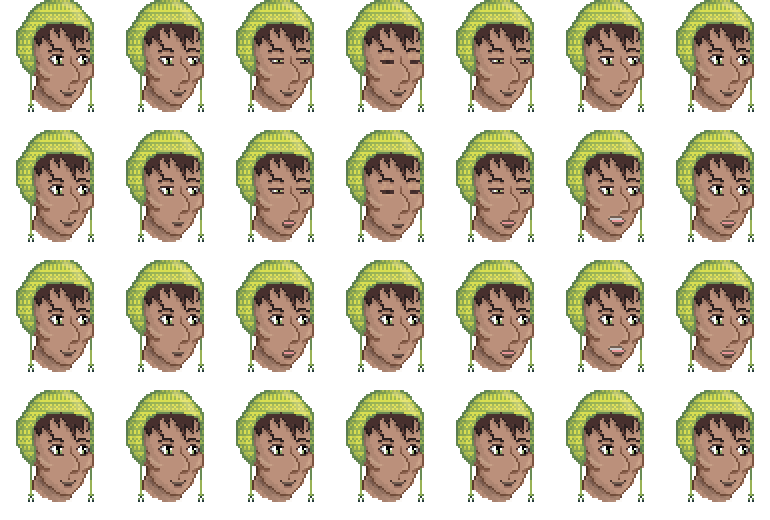
\includegraphics[scale=0.4]{cacamboFaceAnimation}
\centering
\caption{sprite de dialogue de Cacambo}
\end{figure}

\begin{figure}[H]
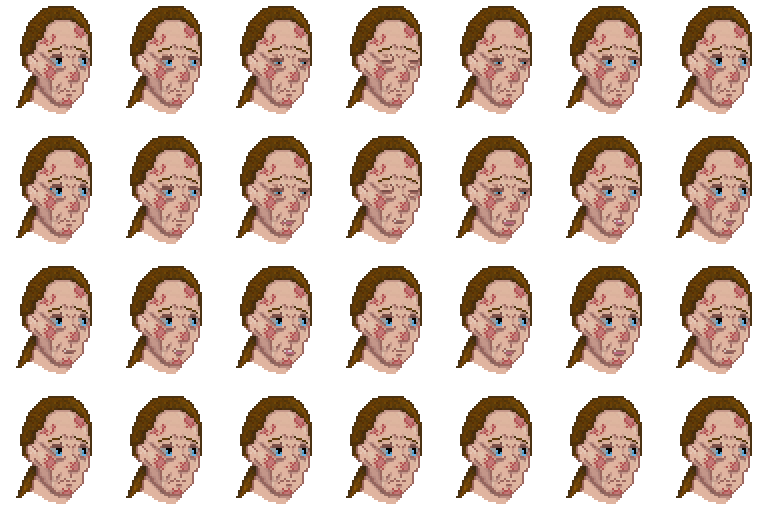
\includegraphics[scale=0.4]{panglossSyphilisFaceAnimation}
\centering
\caption{sprite de dialogue de Pangloss atteint de la syphilis}
\end{figure}

\begin{figure}[H]
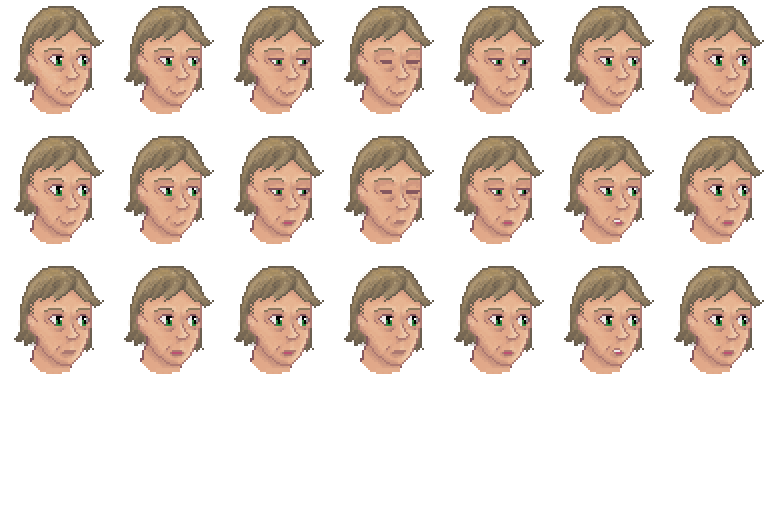
\includegraphics[scale=0.4]{jacquesFaceAnimation}
\centering
\caption{sprite de dialogue de Jacques}
\end{figure}

\begin{figure}[H]
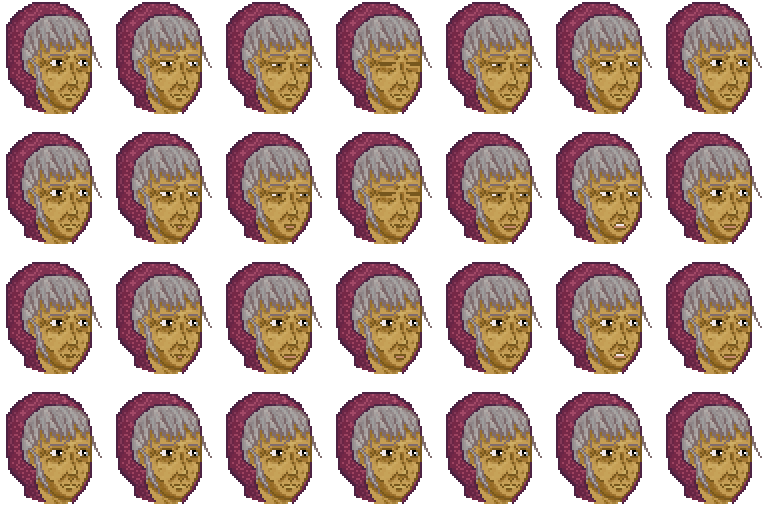
\includegraphics[scale=0.4]{vieilleFaceAnimation}
\centering
\caption{sprite de dialogue de la vieille}
\end{figure}

\begin{figure}[H]
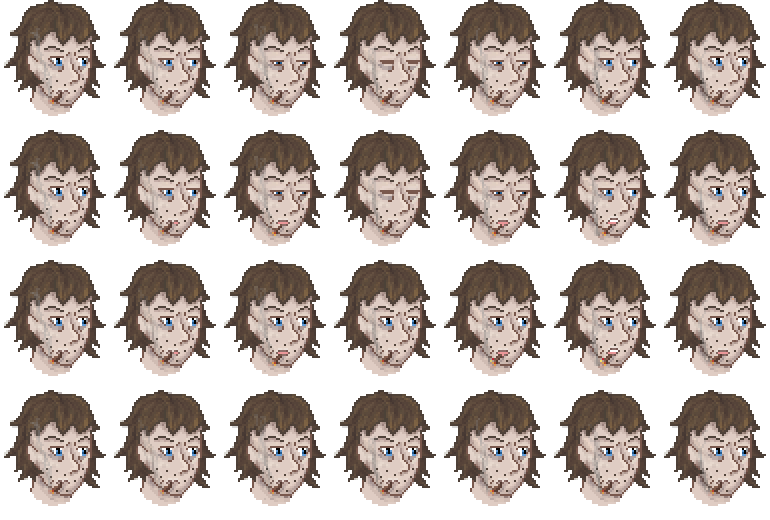
\includegraphics[scale=0.4]{martinFaceAnimation}
\centering
\caption{sprite de dialogue de Martin}
\end{figure}

\begin{figure}[H]
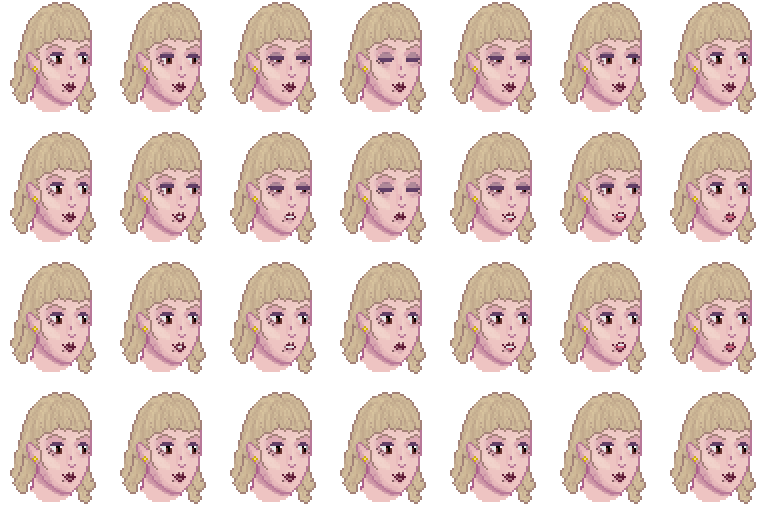
\includegraphics[scale=0.4]{marquiseFaceAnimation}
\centering
\caption{sprite de dialogue de la marquise de Parolignac}
\end{figure}

\newpage
\textit{Note:} Les extraits de code présentés sont des extraits du code source comprenant les passages les plus importants, ils ne sont pas complets.

\subsection{Système général}
	Avant toute chose, il a fallu concevoir un système qui permette d'atteindre diverses variables au travers de tous les outils du jeu. C'est pourquoi l'objet \textit{globals} (présent dans globals.js), une variable globale a été créée. Cet objet stocke toutes les variables afin d'y avoir accès facilement sans devoir se soucier des scopes des différentes classes et de leur méthodes.\\
 
 Afin d'étendre les possibilités futures de diffusion du projet, une option de traduction a été pensée dans le code de départ. Il s'agit d'un chiffre ( 0 pour le français, 1 pour l'anglais, ... ) stocké dans l'objet mentionné au paragraphe ci-dessus. Grâce à cette variable, la fonction de dialogList.js retourne les textes figurants dans le jeu dans leur bonne version. \\
 \begin{lstlisting}[language=JavaScript]
 function setDialog(langue){
    switch(langue){
        case 0 : 
        globals.dialogs.myChar=["Bonjour"];
    break;
        case 1:
        globals.dialogs.myChar=["Hello"];
		break;
 	}
 }
\end{lstlisting}
\textit{Exemple de la fonction traductrice pour le dialogue d'un personnage quelconque}

\subsection{Gestion des states du jeu}
%qu'est-ce qu'une state, comment ça marche etc...\\\\
Les states, propres à Phaser, représentent une section du jeu. Chaque objet State a son lot de méthodes, à savoir \textit{preload()}, \textit{create()}, \textit{update()} et \textit{render()}. L'utilisation de ces fonctions va être décrite dans les paragraphes ci-dessous.

\subsubsection{Boot et Preload}
%boot fait démarrer le jeu, preload pour les assets etc...
La state "Boot" fait démarrer le jeu. Elle déclenche la state "Preload". Preload est une state qui utilise uniquement la méthode \textit{preload()}, qui sert à associer tous les assets du jeu à un nom et les stocker dans le cache pour pouvoir les utiliser dans le code. Une fois tous les éléments stockés, la state "Menu principal" est enclenchée. Le choix d'utiliser une unique state pour ce travail permet une meilleure organisation au sein du code.
\subsubsection{Menu Principal}
%expliquer la fonction avec les boutons, dans un premier temps elle est avec une sprite sheet pour chaque langue, éventuelle amélioration.\\
La state "Menu principal" permet au joueur de lancer le jeu ou d'en modifier la langue. Les boutons qui permettent de faire une action sont des objets Phaser. L'ensemble des boutons est initié dans une seule fonction. Cette fonction dépend de la langue que le joueur a choisi. Chaque bouton a sa propre spritesheet, ce qui pourrait poser problème au niveau de la taille et du temps pour les dessiner si d'autres langues sont ajoutées. Une option serait de générer dans le code, les textes dans les boutons à la place de les dessiner à la main.
\begin{figure}[H]
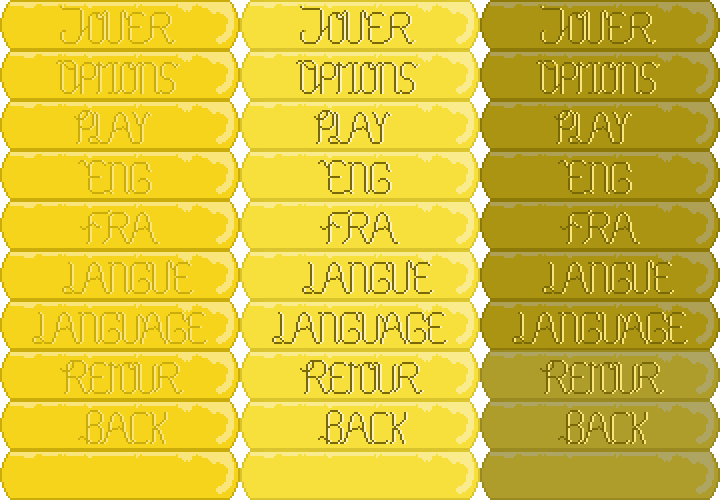
\includegraphics[scale=0.3]{boutons}
\centering
\caption{Spritesheet des boutons utilisés dans le menu}
\end{figure}
\subsubsection{Game}
%toutes les fonctions agissent ici, dans la partie create de phaser.
La state "Game" utilise les méthodes \textit{create()} et \textit{update()}. Dans la méthode \textit{create()}, toutes les actions de jeu sont initiées : le terrain et le personnage sont initiés et les textes du jeu sont traduits.
\begin{lstlisting}[language=JavaScript]
var gameState = {
    create: function(){
        setDialog(gameRef.main.langue);
        createMap1();
        globals.terrainManager.initMap(globals.maps.chateau,true);
        initPlayer(1182,1152)
    },
    update: function(){
        updatePlayer();
        globals.terrainManager.update();
    }
};
\end{lstlisting} 
\textit{Extrait du code de la state "Game".}\\\\
La méthode \textit{update()} est une fonction qui utilise \textit{requestAnimationFrame}. Sont présentes dans cette méthode, toutes les fonctions qui servent à interagir avec le joueur, c'est à dire la détection de la collision, les changements de maps au contact d'une zone de warp et l'apparition des bulles de dialogues des personnages non-jouables quand le joueur les approche. La fonction qui sert à faire marcher le joueur est aussi présente dans la fonction \textit{update()}.
\subsubsection{Battle}
La state "Battle" est utilisée lors des combats pour initier l'interface de combat. Une nouvelle state est utilisée car il est plus facile de créer un contenu visuel à partir d'une state vide que de modifier une state déjà existante. En effet, la state de combat ne requiert pas une détection de collision ni la création de personnages non-jouables.\\

Une map de fond est initiée dans la méthode \textit{create()}, ainsi que les personnages à l'écran et leur barres de vie. Le combat est ensuite géré par une classe, textit{battleManager}, dont le fonctionnement va être décrit plus loin.
\subsubsection{Transition avec texte}
Cette state sert uniquement à afficher du texte. Une fonction est passée en argument lorsqu'on fait appel à cette state qui l'exécutera. Cette state est une alternative narrative aux cinématiques, trop difficiles à programmer.
\begin{figure}[H]
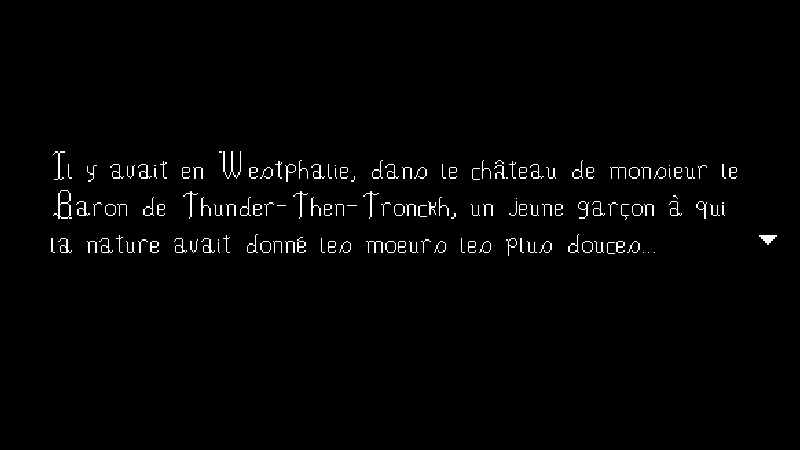
\includegraphics[scale=0.33]{introScreen}
\centering
\end{figure}  
\subsection{Joueur}
%expliquer les déplacements, les directions , les interactions etc...
Le joueur est un sprite qui peut se déplacer lorsqu'une touche directionnelle est enfoncée. Ces déplacements sont activés uniquement quand la propriété "canMove" = true. Cette propriété sert à ce que le personnage ne puisse pas se déplacer pendant les dialogues. Le sprite possède 4 animations de marche qui sont jouées quand l'image se déplace.\\
\begin{figure}[h]
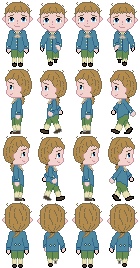
\includegraphics[scale=0.5]{candideSprite}
\centering
\caption{le sprite du joueur avec les différentes frames des animations de marche}
\end{figure}


Les déplacements sont détectés dans la fonction \textit{updatePlayer()} appellée dans la state "Game".\\


Ce sprite possède un corps physique (spécificité de Phaser) qui permet les collisions avec son environnement.


Le sprite possède également de la vie et des attaques, qui vont être utilisées durant les combats. 
\subsection{Les pnjs}
%expliquer la classe, la bulle (classe) 
%les interaction avec le joueur etc.
\subsubsection{Personnages normaux : La classe \textit{Pnj}}
Les pnjs sont une nouvelle classe étendue de la classe sprite de Phaser. Pour créer un nouveau pnj, il faut utiliser :\\
 \begin{lstlisting}[language=JavaScript]
var myChar = new Pnj(x,y,key,frame,name,dialogs,faceAnimKey);
\end{lstlisting}
Voici l'explication de ces arguments:
\begin{itemize}
\item \textbf{x,y}: Définissent la position du sprite.
\item \textbf{key} : Référence de la spritesheet sous forme de string.
\item \textbf{frame} : Numéro qui définit la frame affichée. ( habituellement 0 pour avoir le personnage de face) 
\item \textbf{name} : Nom du personnage sous forme de string.
\item \textbf{dialogs} : Variable contenant les répliques du personnage.
\item \textbf{faceAnimKey} : Référence à la spritesheet des animations pendant un dialogue sous forme de string.
\end{itemize}
\paragraph{}

Chaque pnj a une méthode \textit{update()} qui permet de détecter le joueur et créer une interaction avec lui. Le code regarde si le rectangle formé par le sprite du joueur intersecte un autre rectangle plus grand, qui englobe le pnj. Si c'est le cas et que le phylactère du pnj n'est pas encore à l'écran, le personnage crée une bulle. Lorsque la bulle est affichée, le joueur peut appuyer sur "enter" et faire démarrer le dialogue.\\

Cette méthode de détection de bulle a été codée avec des "if" et beaucoup de variables booléennes. Une amélioration est peut-être possible avec des signaux, une spécificité de Phaser, qui permettent l'appel d'une fonction lorsque qu'un événement est déclenché.\subsubsection{Ennemis : La classe \textit{Ennemy}}
Les ennemis sont une classe étendue de la classe Pnj. Ce sont des pnjs dotés de points de vie et d'attaques pour pouvoir les utiliser lors de combats. Ils ont une propriété importante : \textit{isAlive}, un booléen qui détermine si un combat peut être lancé et permet de mettre fin à un combat lorsque l'ennemi est défait. Chaque ennemi possède une méthode \textit{turn()} utilisée lors d'un tour au combat et une méthode \textit{startCombat()} qui fait basculer le jeu sur la state de combat. Cette méthode sert à définir une cible aléatoire parmi les cibles présentes, choisir une attaque aléatoire et lancer l'attaque sur la cible choisie. Cette méthode renvoie aussi un message qui sera afficher pendant le combat, en fonction de l'attaque choisie.
\subsection{Les bulles : La classe \textit{Bubble}}
 Chaque bulle affichée à l'écran est composée de trois parties, le fond, le texte et un triangle animé. Les bulles jouent plusieurs rôles. Elles peuvent indiquer un dialogue mais aussi permettre au joueur de rentrer dans une nouvelle map (grâce à la méthode \textit{goToHouse()}) lorsqu'il y a un élément tel qu'une porte que le joueur doit ouvrir. La détection des zones de warps à bulle est programmée à l'aide de boucles et de "if". Le code pourrait être simplifié à l'aide de signaux Phaser.
\begin{figure}[H]
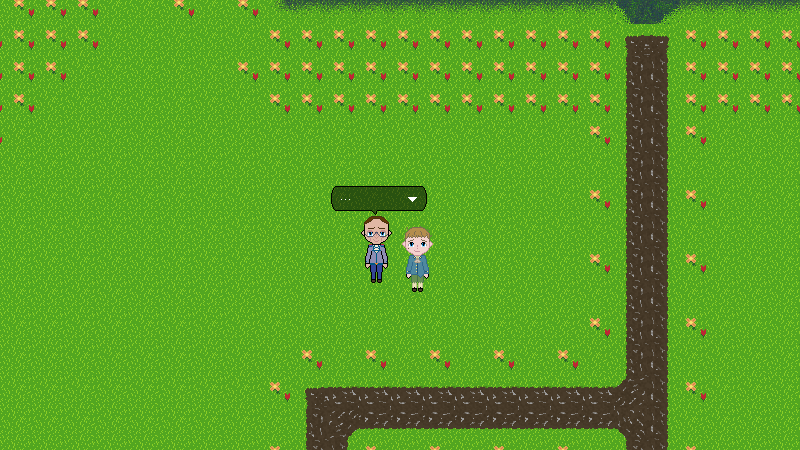
\includegraphics[scale=0.5]{bulleDialog}
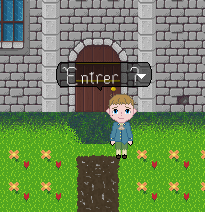
\includegraphics[scale=0.5]{bulleMaison}
\centering
\caption{Exemples de phylactères}
\end{figure}
\subsection{Les attaques : La classe \textit{Attaque}}
Les attaques des objets de la classe \textit{Attaque}. Elles sont utilisées par le joueur et les ennemis lors des phases de combats. Pour créer une attaque il faut utiliser : 
\begin{lstlisting}[language=JavaScript]
var myAttck = new Attaque(name,pdg,cEff,minPdg);
\end{lstlisting} 
Les arguments on la fonction suivante : 
\begin{itemize}
\item \textbf{name}: Nom de l'attaque.
\item \textbf{pdg} : Abréviation de points de dégâts. Le nombre que l'attaque inflige lors de sa première utilisation.
\item \textbf{cEff} : Abréviation de coefficient d'efficacité, définit de combien les points de dégâts diminuent après chaque utilisation.
\item \textbf{minPdg} : Nombre de dégâts minimal que l'attaque inflige.
\end{itemize}
\paragraph{}

Chaque attaque possède la méthode \textit{nextTurn()}, qui recalcule les points de dégâts en divisant les points de dégâts actuels par le coefficient s'ils ne sont en dessus du minimum fixé.\\

Elles possèdent aussi les méthodes \textit{normal(cible)}, \textit{rate(cible)} et \textit{coupCritique(cible)} qui infligent différent dégâts ( Les dommages sont multipliés par 1.5 quand l'attaque est critique. L'attaque ne fait rien lorsqu'elle rate.)\\
Ces méthodes sont utilisées dans la méthode \textit{turn(cible)}, qui choisit aléatoirement une de ces méthodes et l'applique sur la cible choisie. \\

Les attaques possèdent encore deux méthodes qui distribuent de l'information textuelle qui sera utilisée lors des combats. La méthode \textit{info()} indique le nombre de dommages que l'attaque cause. La méthode \textit{desc()} retourne un string en fonction de ce qu'il s'est passé lors du tour.
\subsection{Les barres de vie: La classe \textit{Healthbar}}
Les barres de vies sont des objets graphiques qui s'adaptent en fonction du nombre de points de vie attribués à un personnages. Elle sont en réalité composées de 3 éléments, un contenant vide, le remplissage rectiligne et le remplissage curviligne près du contenant. Il était plus facile de le dessiner ainsi car l'homothétie posait problème lorsqu'il ne restait que quelques hp. \\

A chaque tour, en fonction du nombre de points de vie du personnage, la partie colorée se réduit grâce à une homothétie sur la composante x de facteur nouvelle vie / vie maximum.  Les sprites sont en teintes de gris, pour permettre une coloration en fonction du nombre de points de vie : vert quand les hp sont au dessus de la moitié du maximum, orange quand ils sont au dessus d'un quart du maximum et rouge quand ils sont en dessous. Quand tous les points de vies sont éliminés, le personnage est défait et l'animation de la partie curviligne de l'animation se déclenche.

\begin{figure}[H]

\includegraphics{health}

\includegraphics{healthP2}
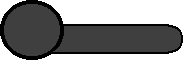
\includegraphics{healthBar}
\caption{Les trois parties de la barre de vie}
\end{figure}
\subsection{Les objets de terrain : Les classes \textit{CustomMap} et \textit{Warp}}
Cette section regroupe deux petits objets traitant du terrains, d'où leur regroupement.\\

Les customMaps sont des objets qui stockent de l'information de terrain. Ils sont utilisés dans le \textit{terrainManager}. Pour déclarer un objet customMap, il faut utiliser : 
\begin{lstlisting}[language=JavaScript]
var myCustomMap = new CustomMap(key,tilesets,layerKeys,music);
\end{lstlisting} 

Les arguments remplissent les fonctions suivantes : 
\begin{itemize}
\item \textbf{key}: Référence de la map sous forme de string.
\item \textbf{tilesets} : Array contenant le nom des tilesets utilisés pour la map.
\item \textbf{layerKeys} : Le nom des couches de la map.
\item \textbf{music} : La référence à la musique associée à la map. Il est automatiquement assigné à undefined si l'argument n'est pas rempli.
\end{itemize}
L'argument music n'est pas encore pris en compte par le code car la musique n'a pas encore été créée. Il est présent pour les utilisations futures. \\

Chaque objet CustomMap possède une clé \textit{plus} qui permet une définition externe (via Tiled) de certains paramètres comme les coordonnées des pnjs et celles des warps. Chaque objet possède également deux méthodes permettant d'ajouter des pnjs et des warps aux clés correspondantes.\\

Dans le code conçu initialement, chaque objet CustomMap était dépendant de toutes ses composantes y compris les pnjs et les warps. Le problème étant qu'après avoir intégré la clé \textit{plus}, les pnjs/waprs étaient aussi dépendant de l'objet CustomMap! Donc impossible de créer l'un ou l'autre, d'où la nécessité d'utiliser des méthodes, une fois que tous les objets ont été créés. \\ 


Les Warps sont également des objets de données. Voici comment déclarer un warp: 

\begin{lstlisting}[language=JavaScript]
var myWarp = new Warp(isHouse,toMap,newX,newY,x,y,tileWidth,tileHeight,text);
\end{lstlisting} 
Un Warp est une zone rectangulaire qui permet le changement de map lorsque le sprite du joueur l'intersecte. Les arguments pour déclarer un warp exercent les fonctions suivantes : 
\begin{itemize}
\item \textbf{isHouse}: Booléen servant à définir si le warp s'active directement ou laisse apparaître un phylactère quand le joueur l'intersecte pour l'activer manuellement.
\item \textbf{toMap} : Nom de la variable contenant un objet CustomMap pour la nouvelle map où le joueur sera amené.
\item \textbf{newX,newY} : Les coordonnées où le sprite du joueur est affiché sur la nouvelle map.
\item \textbf{x,y} : Les coordonnées du haut à gauche du rectangle qui compose l'objet Warp.
\item \textbf{tileWidth,tileHeight} : La largeur et longueur du rectangle en terme de tile de 32x32 pixels. Pour exprimer un rectangle d'une largeur de 64 pixels, il faut utiliser 2 pour tileWidth.
\item \textbf{text}: Le texte affiché dans la bulle du personnage si le Warp doit être activé manuellement. Exemple : "Entrer?"
\end{itemize}
\subsection{Gestion des dialogues : La classe \textit{dialogManager}}
%expliquer la police de caractères, la dynamique des choix, l'objet %manager , la syntaxe (les arrays avec les callbacks etc...)
Tout affichage de texte est géré par la classe \textit{dialogManager} et ses méthodes. 
Chaque morceau de texte doit avoir une syntaxe précise pour pouvoir être affiché grâce à cette classe. Le texte doit être un array qui contient des strings ou des autres arrays.
\begin{lstlisting}[language=JavaScript]
	var txtSimple = ["texte simple"];
	var txtCallback = [
		["texte simple avec callback",function(){}]
	];
\end{lstlisting}
\textit{Exemple de la syntaxe d'un texte simple et d'un texte suivi d'une callback}\\
\begin{lstlisting}[language=JavaScript]
	var txtChoix = [
		[
			"action avec choix",
			["choix 1","choix 2"],
			[function(){callback 1},function(){callback 2}]
		]
	];
\end{lstlisting} 
\textit{Exemple de syntaxe pour un texte qui comporte des choix}
\begin{figure}[H]
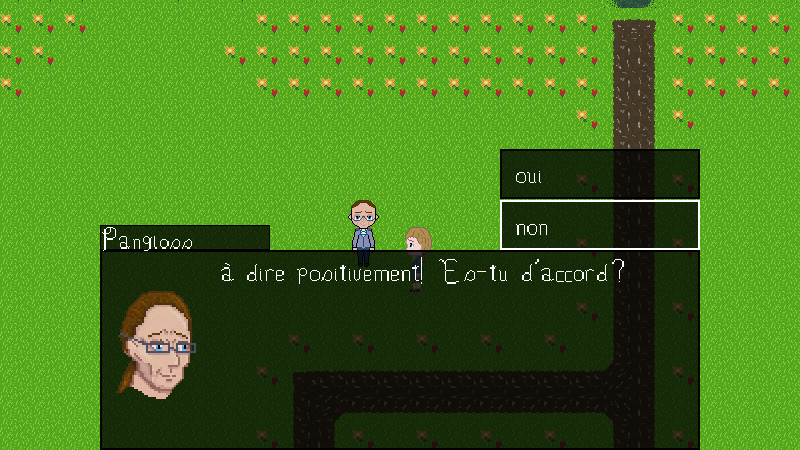
\includegraphics[scale=0.33]{choix}
\centering
\caption{Exemple d'un choix onéreux}

\end{figure}
\subsubsection{méthode \textit{start()}}
Cette méthode affiche une boîte de dialogue standard à l'écran et crée un objet bitmapText vide. Cet objet est un élément graphique de Phaser qui permet d'afficher du texte avec une police choisie au préalable, en l'occurrence la police créée pour ce projet.
\subsubsection{méthode \textit{displayText()}}
\begin{lstlisting}[language=JavaScript]
displayText(texts,index,isDialog,faceAnim,battleDesc)
    if(typeof texts[index] == "string"){
        var textArray = texts[index].split(" "); 
    }
    else {
        var textArray = texts[index][0].split(" ");
        this.texts = texts;
        this.index = index;
    }

    var compteurMots = 0;

    this.bmpText.text = "";

    this.wordTimer = game.time.create();

    this.wordTimer.repeat(100,textArray.length,function(){
        this.bmpText.text += textArray[compteurMots] + " ";

        if(this.bmpText.text.length >= 184){
            this.wait(isDialog,false,false);
            this.wordTimer.pause();
        }
        compteurMots ++;
    },this);
  
        if(typeof texts[index] == "string"){
            this.wordTimer.onComplete.add(function(){
                this.wait(isDialog,true,null,false);
            },this); 
        }
        else if(texts[index].length == 2 ){
            this.wordTimer.onComplete.add(function(){
                this.wait(isDialog,true,texts[index][1],false);
            },this);
        }
        else{
            this.wordTimer.onComplete.add(function(){
                this.wait(isDialog,false,null,true);
            },this);
        }
    
    this.wordTimer.start();

}
\end{lstlisting} 
\textit{Extrait de la méthode displayText()}\\
Cette méthode sert à afficher les mots un par un. Voici ce que représente les arguments:\\
\begin{itemize}
\item \textbf{texts}: La variable qui contient le texte à afficher.
\item \textbf{index} : L'index à partir du quel se trouve le texte à afficher.
\item \textbf{isDialog} : Booléen servant à afficher une animation spéciale si c'est un dialogue.
\item \textbf{faceAnim} : La référence de la spritesheet à animer lors d'un dialogue.
\item \textbf{battleDesc} : Objet de donnée qui est utilisé lors des combats. Comprend les clés booléennes \textit{is,callback} (qui définissent si le texte doit s'en aller automatiquement et s'il contient une callback) et la clé \textit{time} (qui définit le nombre de milisecondes avant que le texte ne s'efface).
\end{itemize}
\textit{Note:}L'usage de \textit{isDialog} et \textit{battleDesc} n'est pas présent dans l'extrait ci-dessus.\\

Si le texte est un dialogue, l'image de la tête du personnage est ajoutée à la boîte de dialogue et l'animation du personnage qui parle est lancée.
Cette méthode sépare ensuite le texte d'entrée en array (\textit{textArray}) et initialise un compteur à 0. Elle crée un timer Phaser, qui ressemble dans son fonctionnement à un \textit{setInterval()}. Toutes les 100 milisecondes, un mot est ajouté à l'élément graphique \textit{this.bmpText} et le compteur est incrémenté jusqu'à ce que le timer ait fait l'opération autant de fois que la longueur de \textit{textArray}. Si le nombre de caractères présents dans l'affichage graphique dépasse 184, le programme met en pause le timer et lance la méthode \textit{wait()}, pour éviter de déborder de la boîte de dialogue.\\

 Quand le timer a terminé d'afficher tous les mots, il lance la méthode \textit{wait()} en fonction du type de texte affiché. Si le texte a un argument battleDesc, la méthode \textit{stop()} est appelée directement lorsque le timer est terminé.\\
 
Finalement, cette méthode enclenche le timer ( il n'a que été créé auparavant).
 
\subsubsection{méthode \textit{wait()}}
\begin{lstlisting}[language=JavaScript]
wait(isDialog,isLast,callback,isQuestion){ 
    input.enter.onDown.addOnce(function(){ 
    	if(!isQuestion){
     	   if(isLast && callback != null){
       	     	callback();
       	 	}
        	else if(isLast){
            	this.stop(isDialog,true);
        	}
        	else{
            	this.resume(isDialog);
        	}
    	}
    	else{
        	this.question(this.texts,this.index);
    	}
	},this);
}
\end{lstlisting} 
\textit{Extrait de la méthode wait()}\\ Cette méthode est un relai qui demande l'appui de la touche "enter" pour continuer quoi que se soit. Voici à quoi servent les nouveaux arguments: 
\begin{itemize}
\item \textbf{isLast} : Booléen servant à fermer le dialogue s'il est complètement affiché.
\item \textbf{callback} : Une fonction callback qui est appelée à la place de la méthode \textit{stop()}
\item \textbf{isQuestion}: Booléen servant à appeler la méthode \textit{question()} si le texte contient des choix.
\end{itemize}
\paragraph{}
Cette méthode dessine et anime un petit triangle d'animation pour signaler au joueur que le script attend une action de sa part. Si le texte affiché est un dialogue, l'animation du personnage est changée : Il cligne simplement des yeux. Cette méthode utilise un signal Phaser. Quand la touche enter est pressée, une méthode est appelée en fonction des besoins du texte qui doit être affiché.
\subsubsection{méthode \textit{resume()}}
Cette méthode prend l'argument \textit{isDialog} et relance si c'est le cas l'animation du personnage qui parle. Elle supprime le triangle animé, remet à zéro le contenu de bitmapText et relance le timer de la méthode \textit{displayText()}:

\subsubsection{méthode \textit{question()}}
\begin{lstlisting}[language=JavaScript]   
question(texts,index){I
    for(var k=0;k<texts[index][1].length;k++){
        var answerBox = game.add.image(0,0,"answerBox");
        answerBox.alignTo(this.dialBox,Phaser.TOP_RIGHT,0,(k*50)+k*1);
        
        var answer = game.add.bitmapText(0,0,"candideFont",texts[index][1][k],50);
        answer.alignIn(answerBox,Phaser.LEFT_CENTER,-15,-10);
        
        this.answerList.push(answer);
        this.answerBoxes.push(answerBox);
    }
    this.selectionBox = game.add.sprite(this.answerBoxes[0].x,this.answerBoxes[0].y,"selection");
    this.selection(texts,index);
}
\end{lstlisting} 
Cette méthode fonctionne à l'aide des arguments \textit{texts} et \textit{index} précédemment mentionnés. Elle supprime le triangle animé, mets à zéro deux arrays contenant les boîtes de réponses ainsi que ces dernières. Ensuite, grâce à une boucle, elle crée les éléments graphiques des réponses (la boîte et le texte). Une fois cela terminé, elle ajoute un sprite en forme de cadre sur la première réponse. Il permet au joueur de voir la réponse qu'il souhaite sélectionner. La méthode \textit{selection()} est ensuite appelée.

\subsubsection{méthode \textit{selection()}}
\begin{lstlisting}[language=JavaScript]
selection(texts,index){
    input.enter.onDown.removeAll(this);
    input.up.onDown.removeAll(this);
    input.down.onDown.removeAll(this);
    
    var max = this.answerBoxes.length;
    
    input.up.onDown.addOnce(function(){
        if(this.selectionBox.y > this.answerBoxes[max -1].y){
            this.selectionBox.y -=51;
        }
        this.selection(texts,index);
    },this);
    
    input.down.onDown.addOnce(function(){
        if(this.selectionBox.y < this.answerBoxes[0].y){
            this.selectionBox.y +=51;
        }
        this.selection(texts,index);
    },this);
    
    input.enter.onDown.addOnce(function(){
        input.up.onDown.removeAll(this);
        input.down.onDown.removeAll(this);
        for(let k=0;k<this.answerBoxes.length;k++){
            if(checkSpriteOverlap(this.selectionBox,this.answerBoxes[k])){
                texts[index][2][k]();
            }
        }
        for(let d=0;d<this.answerBoxes.length;d++){
            this.answerBoxes[d].destroy();
            this.answerList[d].destroy();
        }
        this.selectionBox.destroy();
    },this);
}
\end{lstlisting} 
Cette méthode permet au joueur de choisir une option lorsqu'il est confronté à un choix. Il peut, à l'aide des touches directionnelles verticales,  déplacer le sprite cadre. Lorsqu'il appuie sur enter, la callback associée à la réponse se déclenche. \\

Cette méthode fonctionne  de la manière suivante : premièrement, elle supprime toutes les callbacks associées au signal de chaque input pressé. Ensuite, pour chaque input de verticalité, la méthode ajoute une callback qui ne pourra être utilisée qu'une seule fois lorsqu'une touche est appuyée. Cette callback modifie les coordonnées y du sprite cadre et rappelle la méthode \textit{selection()}. Pour la touche enter, une callback à utilisation unique est aussi associée. Elle supprime les callbacks des touches directionnelles, vérifie quelle réponse est entourée par le cadre grâce à une fonction qui renvoie \textit{true} si les rectangles formés à partir du pourtour de deux sprites s'intersectent. Une fois la réponse déterminée, la méthode lance la callback qui lui est associée et détruit les éléments graphiques qui constituaient l'ensemble des réponses.
\subsubsection{méthode \textit{stop()}}
Cette méthode prend les arguments \textit{isDialog} et \textit{canBulle}. L'argument \textit{canBulle} est un booléen qui détermine si le pnj à qui le joueur parle peut ré-afficher un phylactère à l'écran.\\

Cette méthode supprime tous les éléments graphiques à l'écran y compris les animations des personnages si \textit{isDialog = true}.  Lorsque que les deux arguments de la fonction sont égaux à true, un timer phaser est activé (similaire au \textit{setTimeOut()}) et la bulle du personnage qui vient de parler réapparaît à l'écran après 300 milisecondes. 

\subsubsection{Texte automatique : Les méthodes \textit{startDialog(pnj)}, \textit{startBattleDesc(text,battleDesc)} et \textit{desc(text)}}
Ce sont 3 méthodes utilisées dans le jeu qui appellent les différentes méthodes citées précédemment avec les arguments nécessaires. \\

La méthode \textit{startDialog()} dépend uniquement d'un pnj. Elle affiche le nom du pnj dans un contenant graphique et lance le dialogue en fonction l'index du pnj. \\

la méthode \textit{startBattleDesc()} est utilisée dans les phases de combats et gère les descriptions automatiquement afin que le joueur n'ait pas à intervenir pour que le texte change. \\

La méthode \textit{desc()} sert à afficher du texte pur.  Elle est utilisée dans la state qui s'occupe des transitions avec texte. Cette méthode sera aussi utilisée lorsque l'interaction avec l'environnement sera implémentée.\\


\subsubsection{méthode \textit{endBattleScreen()}}
Cette méthode sert à afficher progressivement une boîte de dialogue ainsi que le texte approprié lorsque le joueur gagne ou perd un combat. Quand le texte est affiché et que le joueur appuie sur enter, le jeu bascule de la state "Battle" à la state "Game". Dans l'état actuel de ce projet, il retourne au même point de départ que lorsque le jeu est lancé mais dans des versions futures, le joueur retrouvera la position qu'il a quittée quand le combat s'est lancé.\\
\begin{figure}[H]
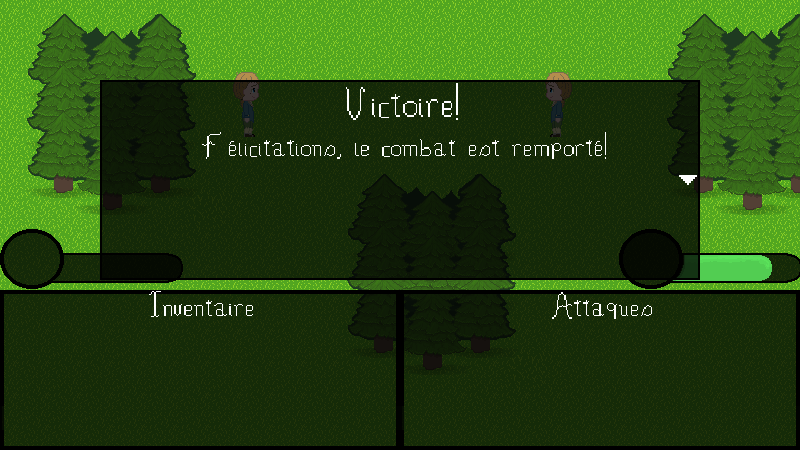
\includegraphics[scale=0.35]{victoire}
\centering
\end{figure}
\subsection{Gestion du terrain : La classe \textit{TerrainManager}}
Le \textit{terrainManager} est un objet qui grâce à ses méthodes, gère les changement de terrains.
\subsubsection{méthode \textit{initMap()}}
\begin{lstlisting}[language=JavaScript]

    initMap(map,collision){ 
        this.currentMap = game.add.tilemap(map.key);

        for(let l in map.tilesets){
            this.currentMap.addTilesetImage(map.tilesets[l],map.tilesets[l]); 
        }

        this.currentLayers = [];
        for(let k of map.layerKeys){

            let layer = this.currentMap.createLayer(k);
            this.currentLayers.push(layer);
        }

        if(collision){
            this.collision = this.currentMap.createLayer("Collision");
            this.currentMap.setCollisionByExclusion([], true, this.collision);
            this.collision.resizeWorld();
            this.collision.visible = false;
        }
        this.currentMap.plus.animation.enable();
        this.currentLayers[0].resizeWorld();

        for(let l in map.pnjs){
            game.add.existing(map.pnjs[l]);
            this.currentPnjs.push(map.pnjs[l]);
        }
        for(let l in map.warps){
            this.currentWarps.push(map.warps[l]);
            this.currentWarps[l].overlap=false;
        }
    }
\end{lstlisting} 
Cette méthode initialise tous les composants du terrain. Elle prend en compte 2 arguments :
\begin{itemize}
\item \textbf{map} : L'objet CustomMap qui contient les données du terrain que l'on souhaite afficher. 
\item \textbf{collision} : Booléen qui définit si le terrain possède une couche nommée "Collision".
\end{itemize}
La couche de collision possède toutes les tiles avec lesquelles le joueur doit rentrer en collision. \\

Cette méthode crée un objet Phaser Map, puis construit visuellement chaque couche avec les tilesets. Les personnages sont ensuite ajoutés et enfin les warps. Chaque carte affichée est enregistrée sous une clé inaccessible en dehors de la méthode une fois que le décor est posé, d'où la nécessité d'utiliser les CustomMaps.
\subsubsection{méthode \textit{clearMap()}}
Cette méthode supprime tous les éléments graphiques de l'écran. Elle réinitialise également les clés \textit{currentLayers}, \textit{currentPnjs} et \textit{currentWarps}.
\subsubsection{méthode \textit{changeMap()}}
Cette méthode s'active lorsque le joueur pose le pied sur un warp. 
Elle crée un fondu enchaîné sur du noir, détruit tout ce qu'il y a a l'écran, reconstruit le nouveau décor puis l'écran noir se fond à nouveau sur le jeu.\\

Lors de la réalisation, le fondu a été programmé en plus des autres méthodes mais il ne marchait qu'à moitié : Même si le personnage bougeait, le rectangle noir qui obstruait la fenêtre de vue restait à la même place! C'est en s'aventurant dans la documentation que des méthodes permettant ces effets ont été découvertes...
%expliquer les maps,collisions, tilesets,calques, warps , l'objet terrainmanager etc... expliquer le fail avec le tween manager pour le fade in et fade out.
%expliquer le problème avec les données dans la map et la solution
\subsubsection{méthode \textit{update()}}
Cette méthode établit la collision entre le joueur et l'environnement ainsi que les personnages composants la scène. Elle vérifie aussi les détections d'intersections avec les warps pour afficher si besoin une bulle.

Il y a eu des problèmes avec les bulles, car dans une première version du code, elles étaient constamment supprimées. C'est expliqué par le fait que le warp pénétré n'était pas retenu et que le code vérifiait pour chaque warp présent dans la map si le joueur était dedans. Comme les conditions étaient vérifiées, la bulle était supprimée aussitôt qu'elle était créée. Le problème a été géré en associant la zone de warp à une variable et de vérifier le contenu de cette variable avant de supprimer la bulle.
\subsection{Gestion des combats : La classe \textit{BattleManager}}
Cette state est responsable des combats du jeu. Elle gère les tours des combats et orchestre les affichages. 
\subsubsection{méthode \textit{init()}}
\begin{lstlisting}[language=JavaScript]

\end{lstlisting} 
\subsubsection{méthode \textit{clearMap()}}
\begin{lstlisting}[language=JavaScript]

\end{lstlisting} 
\subsubsection{méthode \textit{clearMap()}}
\begin{lstlisting}[language=JavaScript]

\end{lstlisting} 
\subsubsection{méthode \textit{clearMap()}}
\begin{lstlisting}[language=JavaScript]

\end{lstlisting} 
\subsubsection{méthode \textit{clearMap()}}
\begin{lstlisting}[language=JavaScript]

\end{lstlisting} 
\subsubsection{méthode \textit{clearMap()}}
\begin{lstlisting}[language=JavaScript]

\end{lstlisting} 
\subsubsection{méthode \textit{clearMap()}}
\begin{lstlisting}[language=JavaScript]

\end{lstlisting} 
\subsubsection{méthode \textit{clearMap()}}
\begin{lstlisting}[language=JavaScript]

\end{lstlisting} 
\subsubsection{Gestions des signaux}
\begin{lstlisting}[language=JavaScript]

\end{lstlisting} 
%expliquer la dynamique de combat, les points de vie etc..

%\subsection{Du code à l'application}
%parler d'éléctron, npm, des packages.json, du favicon, de la fenêtre et des sauvegardes de la partie. (fenêtres)

%\subsection{Publication}
%système de sauvegarde , gitpages

\end{appendices}
\end{document}


